% !TeX root=tukedip.tex
% !TeX encoding = UTF-8
% !TeX spellcheck = sk_SK
\section{Prehľad literatúry}
Pred výberom metódy optického polohovania a navigácie sme museli preskúmať rôzne možnosti. Pozreli sme sa na metódy, ktoré by mohli byť vhodné na navigáciu dronov. Skúmala sa ich použiteľnosť pre mikrodrony.

\subsection{Optický princíp senzorov}
Snímače s optickým princípom sa bežne používajú v mobilnej robotike na navigáciu, lokalizáciu a mapovanie. Tieto senzory zachytávajú informácie z prostredia analýzou svetla a jeho interakcie s povrchmi, čím poskytujú bohaté údaje na presné určovanie polohy robota a plánovanie trajektórie. V tejto časti sa budeme zaoberať rôznymi typmi optických principiálnych snímačov a ich aplikáciami v mobilnej robotike.

Jedným z najčastejšie používaných optických snímačov je kamera, ktorá zachytáva obrázky a videá prostredia. Kamery poskytujú bohaté vizuálne informácie vrátane farby, textúry a tvaru, ktoré možno využiť na detekciu, sledovanie a rozpoznávanie objektov. V našej práci využívame kamery namontované na bezpilotných lietadlách Tello na zisťovanie polohy značiek Aruco a odhadovanie ich súradníc v 3D priestore.

Ďalším dôležitým optickým senzorom je senzor LIDAR (Light Detection and Ranging), ktorý vysiela laserové lúče a meria ich odraz na vytvorenie 3D mapy prostredia. Senzory LIDAR sa bežne používajú v autonómnych vozidlách na vyhýbanie sa prekážkam a mapovanie. Sú však drahé a vyžadujú vysoký výpočtový výkon, čo ich robí menej vhodnými pre malú mobilnú robotiku.
 
Okrem kamier a LIDAR-u patria medzi ďalšie typy snímačov na optickom princípe infračervené snímače, ultrazvukové snímače a snímače času letu. Infračervené senzory merajú odraz infračerveného svetla na detekciu objektov a meranie ich vzdialenosti, zatiaľ čo ultrazvukové senzory vysielajú vysokofrekvenčné zvukové vlny a merajú ich ozvenu na odhad vzdialenosti. Snímače času letu využívajú svetlo na meranie času, za ktorý sa signál odrazí späť, čím poskytujú presné merania vzdialenosti.

Senzory na optickom princípe celkovo zohrávajú kľúčovú úlohu v mobilnej robotike a poskytujú bohaté informácie na navigáciu a lokalizáciu robota. Pochopením rôznych typov senzorov a ich aplikácií môžeme navrhnúť a implementovať efektívne robotické systémy, ktoré môžu fungovať v rôznych prostrediach a scenároch.

\subsection{Vyhýbanie sa prekážkam a orientácia na základe obrazu z kamery}
Jedným z najdôležitejších úloh mobilných robotov je schopnosť vyhnúť sa prekážkam a správne sa orientovať v prostredí. K dispozícii sú rôzne senzory, ktoré umožňujú robotom rozpoznať a vyhnúť sa prekážkam. Okrem senzorov ako LIDAR, ultrazvukových a infračervených senzorov sa dá využiť aj obraz z kamery.

Kamera poskytuje bohaté vizuálne informácie o prostredí a umožňuje robotom získavať informácie o prekážkach a teréne. Existujú rôzne spôsoby, ako využiť obraz z kamery pre navigáciu a vyhýbanie sa prekážkam.

\subsubsection{S vylepšenou neurónovou sieťou}
Jednou zo skúmaných metód na vyhýbanie sa prekážkam a orientáciu pomocou kamery bolo strojové učenie pomocou neurónových sietí \cite{citácia6}. Nakoniec však bola zavrhnutá kvôli časovo a hardvérovo náročným procesom učenia. Táto metóda zahŕňa použitie naučenej neurónovej siete na priradenie približných hodnôt hĺbky každému pixelu na základe polohy objektov z jedného obrazu. Vzory sa dajú naučiť z dvojice LIDAR a digitálnych kamier umiestnených vedľa seba. Zadaním dostatočného počtu týchto naučených dvojíc môže neurónová sieť vytvoriť vzťah medzi pixelmi na obrázkoch a hodnotami hĺbky získanými z LIDAR-u alebo stereokamery.

Sieť sa môže učiť pomocou učenia založeného na LIDAR-e s dohľadom a učenia založeného na stereopároch bez dohľadu na základe pravdepodobnostného princípu. Učenie pod dohľadom je však často príliš prísne a učenie bez dohľadu poskytuje nepresné výsledky. Preto sa odporúča používať poloprevádzkové učenie \cite{citácia7} alebo porovnávať výsledky získané pomocou siete s kalibrovaným systémom detekcie hĺbky počas prevádzky \cite{citácia8}.

Táto metóda získava hodnoty hĺbky z okolia a umiestnenia objektov (množiny pixelov) a vytvára mapu hĺbky podobnú tej, ktorá je znázornená na obrázku 1. Jej presnosť je zatiaľ experimentálna a takýto systém je stále vystavený mnohým chybám. Napriek tomu bol použitý v aplikáciách na riadenie dronov \cite{citácia9}. Hĺbkové mapy na obrázku 1 ilustrujú rozdiel medzi rôznymi metódami a presnosť tejto metódy.

\begin{figure}[ht!]
    \centering
    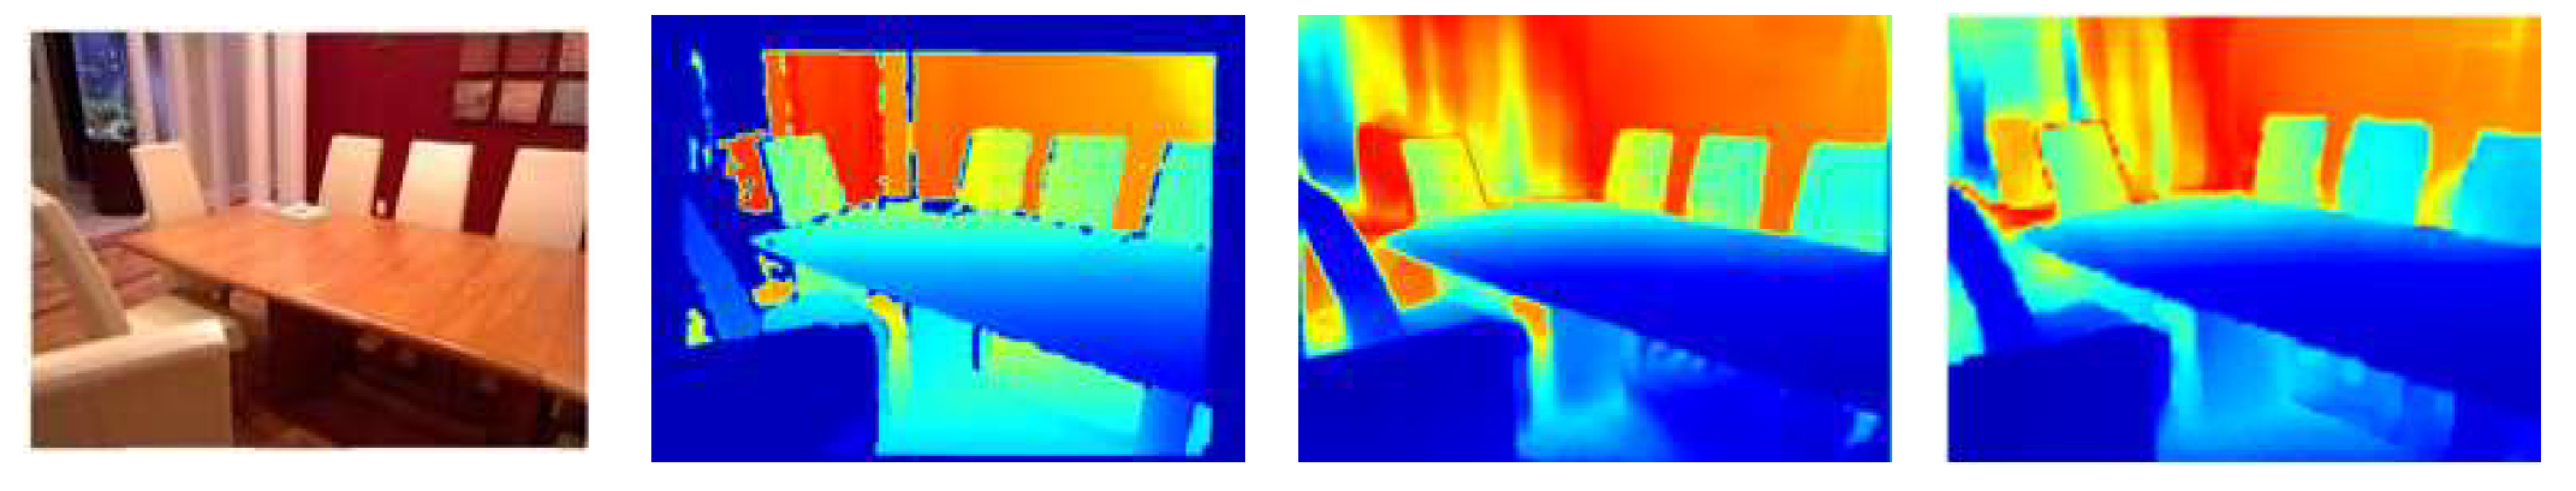
\includegraphics[width=.85\textwidth,angle=0]{figure 2-1.pdf}
    \caption{Načítaný obraz (vľavo), skutočná mapa hĺbky na základe senzorov (vľavo uprostred) a napokon mapa hĺbky vytvorená pomocou Gaussovho modelu (vpravo uprostred) a Laplaceovho modelu (vpravo)}
    \label{o:2-1}
\end{figure}
% Khan, F.; Salahuddin, S.; Javidnia, H. Deep Learning-Based Monocular Depth Estimation Methods—A State-of-the-Art Review. Sensors 2020, 20, 2272. https://doi.org/10.3390/s20082272

Neurónová sieť berie do úvahy niekoľko faktorov:
\begin{itemize}
    \item \textbf{oklúzia}
    \item \textbf{relatívna veľkosť}
    \item \textbf{vrhaný tieň}
    \item \textbf{tieňovanie}
    \item \textbf{vzdialenosť od horizontuň}
    \item \textbf{gradient textúry}
    \item \textbf{lineárna perspektíva}
\end{itemize}
Učenie siete je časovo a zdrojovo náročné. Po vyškolení je výzvou zabezpečiť, aby sieť fungovala v reálnom čase na riadenie dronov bez toho, aby sa stratilo príliš veľa údajov v dôsledku zrýchlenia kalibrácie, čo môže viesť ku kolíziám. Počas pomalého letu sa sieť stále dokáže vyhýbať prekážkam, ale považuje ich len za súbor bodov s relatívnou polohou, nie za presné obrysy.

\begin{figure}[ht!]
    \centering
    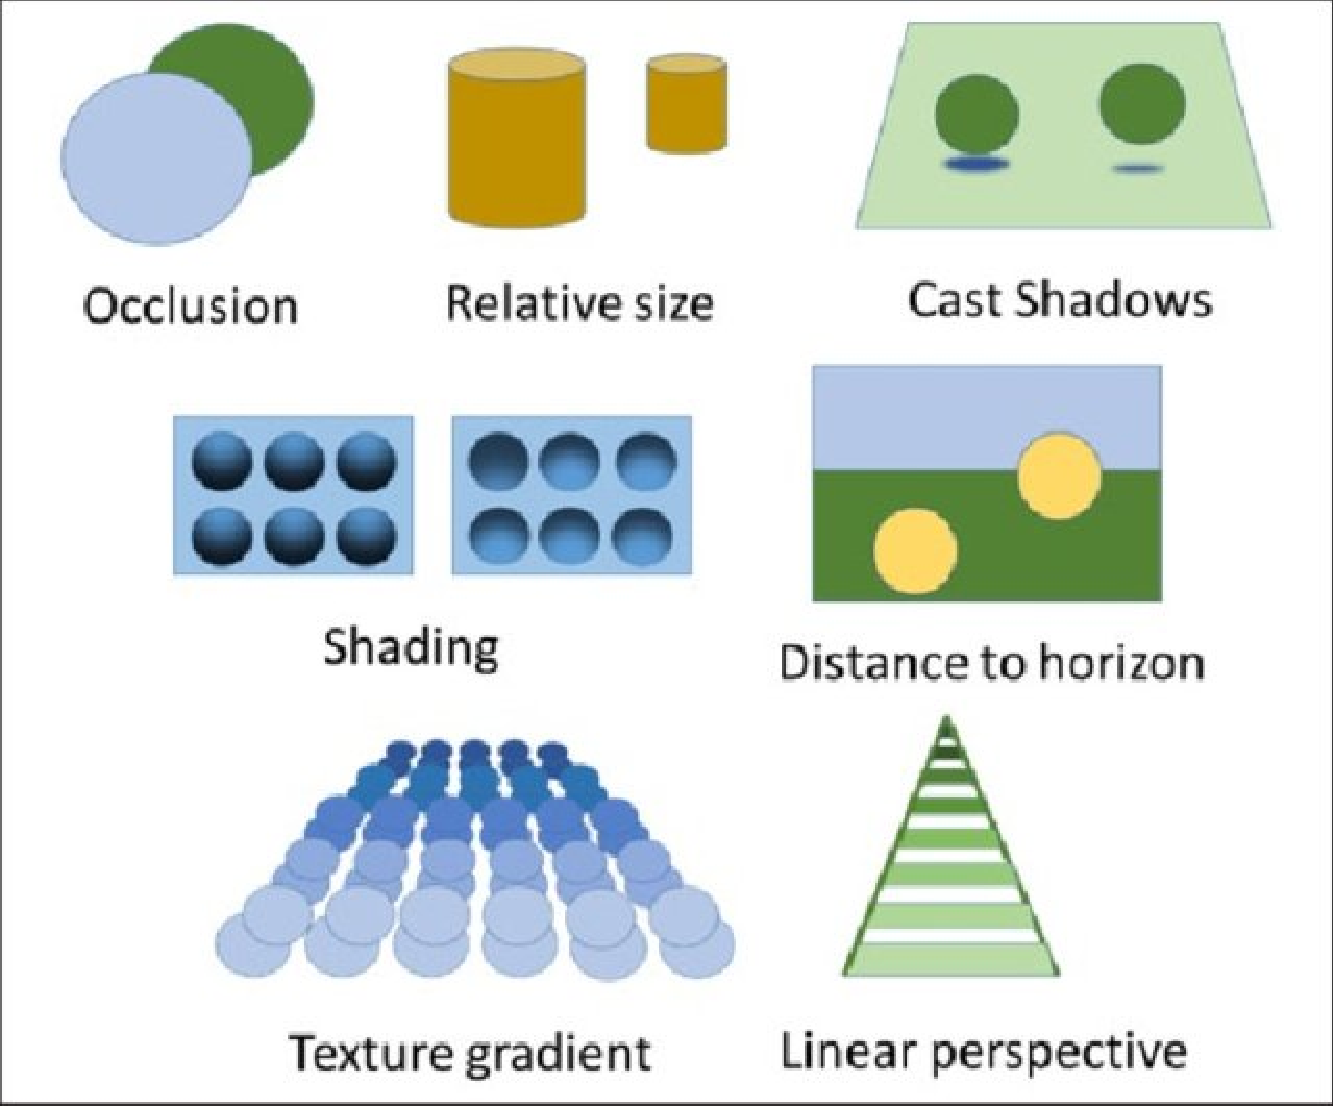
\includegraphics[width=.85\textwidth,angle=0]{figure 2-2.pdf}
    \caption{Faktory zohľadňované pri monokulárnom vnímaní hĺbky}
    \label{o:2-2}
\end{figure}
% Bogdanova, Rositsa & Boulanger, Pierre & Zheng, Bin. (2016). Depth Perception of Surgeons in Minimally Invasive Surgery. Surgical Innovation. 23. 10.1177/1553350616639141. 

\subsubsection{Princíp stereosnímania}
Princíp stereosnímania je široko používaná metóda vnímania hĺbky v počítačovom videní, robotike a príbuzných oblastiach. Zahŕňa použitie dvoch alebo viacerých kamier na snímanie obrazov tej istej scény z rôznych uhlov pohľadu a následné použitie rozdielov v obrazoch na výpočet vzdialeností objektov na scéne. Tento princíp sa uplatňuje pri rôznych úlohách v robotike vrátane rozpoznávania objektov, navigácie a vyhýbania sa prekážkam.

V kontexte bezpilotných lietadiel môže byť princíp stereočočočky užitočným nástrojom na navigáciu a vyhýbanie sa prekážkam. Populárny dron DJI Tello má však napríklad len jednu kameru. V takomto prípade možno obraz z kamery rozdeliť na dve virtuálne kamery, ktoré sa potom môžu použiť na simuláciu stereovidenia. Tento prístup má však svoje obmedzenia a výzvy.

Jednou z hlavných výziev je, že rozlíšenie virtuálnych kamier je nižšie ako rozlíšenie skutočnej kamery. Toto zníženie rozlíšenia môže ovplyvniť presnosť vnímania hĺbky, najmä v prípade vzdialených objektov. Ďalšou výzvou je, že základná vzdialenosť medzi dvoma virtuálnymi kamerami je pevná a nedá sa upraviť, čo môže obmedziť rozsah vzdialeností, ktoré možno presne odhadnúť.

Okrem toho výkonnosť princípu StereoLensing môžu ovplyvniť rôzne faktory, ako sú svetelné podmienky, kalibrácia kamery a oklúzie. Tieto faktory môžu mať za následok chyby vo vnímaní hĺbky, čo môže viesť ku kolíziám alebo nepresnej navigácii.

Vzhľadom na tieto problémy je pochopiteľné, prečo princíp StereoLensing nemusí byť vždy najlepším riešením pre navigáciu dronov a vyhýbanie sa prekážkam. Namiesto toho môžu byť na tieto úlohy vhodnejšie iné techniky, ako napríklad LiDAR, ultrazvukové senzory a vizuálno-inerciálna odometria, najmä v prostredí s náročnými svetelnými podmienkami alebo zložitými štruktúrami.

Na záver možno konštatovať, že hoci je princíp stereosnímania výkonnou metódou na vnímanie hĺbky a úspešne sa uplatňuje v rôznych oblastiach, jeho použitie v kontexte dronov, ako je Tello, je obmedzené z dôvodu použitia iba jednej kamery. V dôsledku toho môže byť potrebné použiť iné techniky snímania v spojení s týmto princípom, aby sa dosiahla presná a spoľahlivá navigácia dronov a vyhýbanie sa prekážkam.
\subsubsection{Na základe pohyblivého obrazu kamery}

\subsubsection{Určovanie polohy pomocou značiek}

\subsection{WebSocket}





